\section{tasks::sumdarks Class Reference}
\label{classtasks_1_1sumdarks}\index{tasks::sumdarks@{tasks::sumdarks}}
Inheritance diagram for tasks::sumdarks::\begin{figure}[H]
\begin{center}
\leavevmode
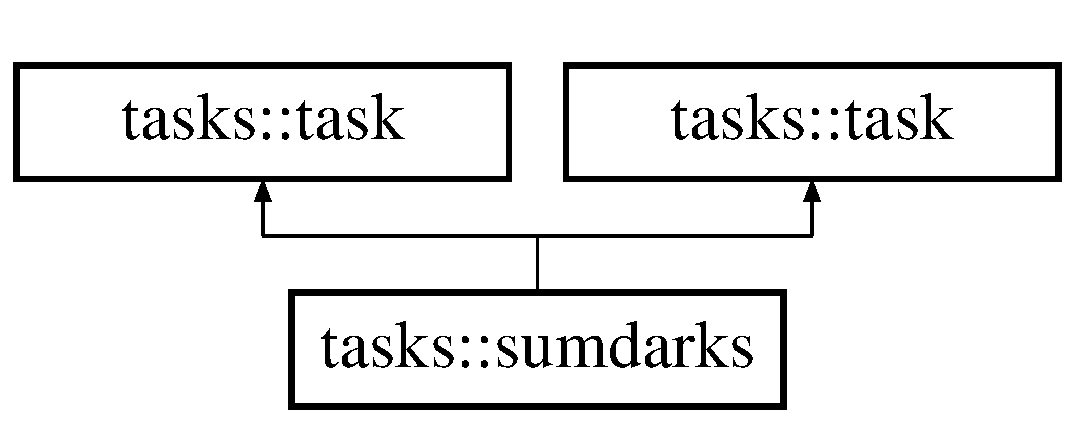
\includegraphics[height=2cm]{classtasks_1_1sumdarks}
\end{center}
\end{figure}
\subsection*{Public Member Functions}
\begin{CompactItemize}
\item 
def \textbf{run}\label{classtasks_1_1sumdarks_0980fff288b35b209f8e661d8c37ec94}

\item 
def \textbf{run}\label{classtasks_1_1sumdarks_0980fff288b35b209f8e661d8c37ec94}

\end{CompactItemize}
\subsection*{Static Public Attributes}
\begin{CompactItemize}
\item 
string \textbf{name} = '{\bfsumdarks}'\label{classtasks_1_1sumdarks_cf155e58f65ea1773b160129c8fe08e1}

\item 
string \textbf{button\-Text} = 'Create combined Darks'\label{classtasks_1_1sumdarks_f5165a7efe16382f349fc701a344c722}

\end{CompactItemize}


\subsection{Detailed Description}


\footnotesize\begin{verbatim}Combine a set of DARKS frames into the combined darks frame. The currently
   implemented method is median filtering of the images.
\end{verbatim}
\normalsize
 



The documentation for this class was generated from the following files:\begin{CompactItemize}
\item 
old/PANICtool-1.0/tasks.py\item 
old/tasks.py\end{CompactItemize}
